\usetikzlibrary{calc}
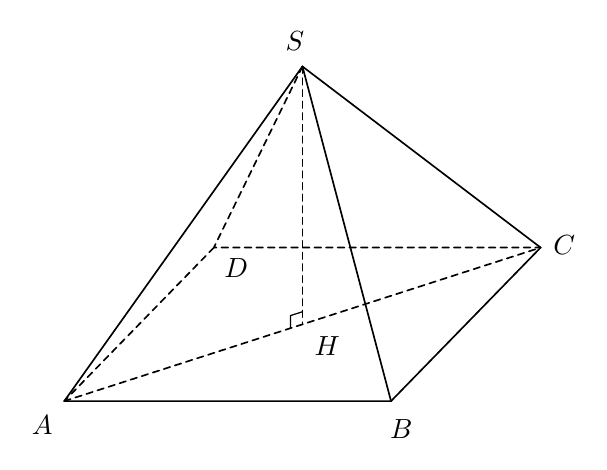
\begin{tikzpicture}[x=1cm,y=1cm,line width=.6pt,line cap=round,line join=round]
  \tikzset{
    gedge/.style={line width=.6pt},
    ghidden/.style={line width=.6pt,dash pattern=on 2.4pt off 1.8pt},
    gdot/.style={circle,fill=black,draw=none,inner sep=0pt,minimum size=1.6pt},
    glabel/.style={inner sep=1.5pt,font=\normalsize}
  }
  \coordinate (A) at (0.70,0.90);
  \coordinate (B) at (4.85,0.90);
  \coordinate (C) at (6.75,2.85);
  \coordinate (D) at (2.60,2.85);
  \coordinate (H) at (3.725,1.875);
  \coordinate (S) at (3.725,5.15);
  \draw[gedge] (S)--(A)--(B)--(C)--cycle;
  \draw[gedge] (S)--(B);
  \draw[ghidden] (S)--(D)--(C);
  \draw[ghidden] (D)--(A);
  \draw[ghidden] (A)--(C);
  \draw[ghidden] (S)--(H);
  \coordinate (R1) at ($(H)+(0,0.16)$);
  \coordinate (R2) at ($(H)+(-0.152,-0.049)$);
  \coordinate (R3) at ($(R1)+(-0.152,-0.049)$);
  \draw[line width=0.45pt] (R1)--(R3)--(R2);
  \node[glabel] at (3.63,5.47) {$S$};
  \node[glabel] at (0.42,0.60) {$A$};
  \node[glabel] at (4.98,0.55) {$B$};
  \node[glabel] at (7.05,2.88) {$C$};
  \node[glabel,below right=2pt] at (D) {$D$};
  \node[glabel] at (4.04,1.60) {$H$};
\end{tikzpicture}
